
\section{Preambles}

\subsection{%Brief definition of t
The algebras $J_{l,n}$ and some key properties}
%\ppm{[you did a great job in your report talk. could drop that in here?]} \bajm{[Yes, I will!]}
In this subsection, we give a brief {review}
%\ppm{[-these words dont really go together.  maybe brief review?]}
of the algebras, $J_{l,n}$, constructed in \cite{KadarYu} and recall some properties of these algebras which will be of use in later sections. For a more detailed description of the $J_{l,n}$ we refer readers to the original reference \cite{KadarYu}. %\bajm{[is the following a good place to start/ levek to pitch at??]}\ppm{[could be. but it all takes time. possibly rely a bit more on the original paper this time around?]}


\mdef   \label{de:Brp}
Fix integers $n,m\geq 0$. 
A Brauer partition of type $(n,m)$ is a pair partition of the set $\{1,\dots, n\}\sqcup \{1',\dots, m'\}$ (we use primed labels to distinguish elements of the two sets). Let $\mathcal{B}(n,m)$ denote the set of all such partitions (observe that $\mathcal{B}(n,m)$ is empty unless $n\equiv m\mod 2$). 

We write $\Brp^{r}(n,m)$ for the subset of  $\Brp^{}(n,m)$ of partitions with at most $r$ pairs of the form $\{i,j'\}$ 
(called propagating lines); and $\Brp^{=r}(n,m)$ for the subset with exactly $r$ propagating lines. 

\mdef   \label{pa:left-right}
A partition, $p \in \mathcal{B}(n,m)$, may be represented by a Brauer diagram as follows. 
A Brauer diagram consists of a rectangular region with unprimed (primed) labels placed on the top (bottom) edge 
%\ppm{[just looking at the arxiv version of KY it looks other way round?]}\bajm{[okay I'll switch to the KY conventions which is primed on the bottom left multiplcation = juxtaposing on top, and $\mathcal{B}(n,m)= n$ on top $m$ on bottom.]}
increasing from left to right, and inscribed curves joining labels which belong to the same part. Curves in a Brauer diagram only intersect transversely, on their interiors, finitely many times, and do not have points of triple intersection. We frequently abuse notation, representing by a Brauer diagram its underlying partition. 

\mdef  \label{de:flip}
We write $p \mapsto p^*$ for the map $*: \Brp(n,m) \rightarrow \Brp(m,n)$ corresponding to 
vertical flip of a diagram, hence swapping primed for unprimed. Examples:
\medskip 

{\centering
\sigone{.41}  \hspace{.32cm}$ \stackrel{*}{\mapsto}$\hspace{.32cm}  \sigtwo{.41}

\sigtwo{.41}  \hspace{1cm}   \sigone{.41}

\medskip }

Observe in particular that there is a copy of the symmetric group $\Sym_n$ (so far just as a set) in $\Brp(n,n)$, indeed it is precisely $\Brp^{=n}(n,n)$, and here the flip takes an element to its inverse in the group. 


\mdef    \label{pa:ground-ring}
Fix a commutative ring $\K$ - by default we will take $\K=\C$. 
%\ppm{[-OK this is good to establish. And it means that for most of the det sections we need to say explicitly that we work over $\C[\xx]$ instead.]}
Fix $\a \in \K$. Let $Br(n,m)$ denote the free $\K$-module with basis 
$\mathcal{B}(n,m)$. Define the Brauer category $Br=Br(\a)$ to be the triple $(\N_{0}, Br(\_, \_), \circ )$, where for $(p_1,p_2)\in Br(n,m)\times Br(m,l)$, composition is defined by linearly extending the formula
\[p_1\circ p_2 = \a^{d_{p_1,p_2}} p_1\# p_2.\]
Here $p_1\# p_2 \in Br(n,l)$ is the resultant Brauer partition determined by vertically juxtaposing any two diagrams for $p_1$ and $p_2$,
with $p_1$ over $p_2$, 
and $d_{p_1,p_2}$ is the number of closed curves in any such juxtaposition. For brevity, we adopt the multiplicative notation $p_1 \circ p_2=p_1 \, p_2$. 

\mdef \label{de:flip2}
The *-map extends to a contravariant functor $(\_)^*:Br(\a)\to Br(\a)$ with $n^*=n$ for objects, and $(\_)^*:Br(n,m)\to Br(m,n)$ is given by linearly extending the map from \ref{de:flip}.

\mdef 
Note that the category $Br$ has a monoidal structure given by $n\otimes m=n+m$ on objects, and where $p_1\otimes p_2$ is the horizontal juxtaposition of diagrams. 

\mdef The {\em height} of a Brauer diagram is defined to be the maximal height of all points of intersection of embedded curves as in \cite[\S2.2]{KadarYu}. If a diagram has no points of intersection, its height is defined to be $-1$.

\mdef The height of a Brauer partition, $p\in \mathcal{B}(n,m)$, is defined to be the minimal height over all diagrams representing $p$. Write $ht(p)$ for the height of $p$.

\mdef   \label{de:Jln}
Fix an integer $l\geq -1$. Let $J_{l}(n,m)$ denote the free $\K$-module with basis 
$$
\Brp_l(n,m) \; := \; \{ p \in \mathcal{B}(n,m) \ | \ ht(p)\leq l\}    .
$$ 
In \cite[Thm. 3.4]{KadarYu} it is proved that for any $(p_1, p_2)\in \mathcal{B}(n,m)\times \mathcal{B}(m,l)$,  $ht(p_1\# p_2)\leq \max(ht(p_1),ht(p_2))$, and thus 
$J_l:=(\N_0,J_l(\_, \_), \circ )$ defines a subcategory of $Br$ for each $l$. 

Following \ref{de:Brp}, let $J_l^p(n,m)$ denote the submodule of $J_{l}(n,m)$ spanned by diagrams with at most $p$ propagating curves, and let $J_l^{=p}(n,m)$ denote the submodule spanned by those exactly $p$ propagating curves.   

Let $J_{l,n}:=J_{l}(n,n)$ denote the endomorphism algebras of $J_l$, with $J^{p}_{l,n}=J^{p}_{l}(n,n)$ and likewise $J^{=p}_{l,n}=J^{=p}_{l}(n,n)$. 
We refer to the $\K$-algebras $J_{l,n}$ as the Kadar-Yu algebras.


\mdef\label{pa:Jlngens} In \cite{KY2} it is proved that $J_{l,n}$ is generated as an algebra by the usual ``cup cap" Temperley-Lieb generators $e_i=\uu_{i,i+1} \uu_{i,i+1}^*$ for $i=1,\dots, n-1$ (using the notation of \ref{cupbasis}), and the elementary transpositions $s_j=(j \ j+1)$ for $j=1,\dots,l+1$ (\textit{i.e.} $s_j \in \Sigma_{l+2}$).

\begin{remark} When $l=-1$, the Category $J_{-1}$ may be identified with the Temperley-Lieb category, since in this case all pair partitions may be realised by diagrams without intersections. 
\end{remark}

\mdef 
Note that the monoidal product $\otimes$ on category $Br$ does not descend to one on $J_{l}$ (unless $l=-1$) since, for instance, $ht(id_n \otimes p)=ht(p)+n$ provided $ht(p)\geq 0$. However, it will be convenient for our aims to utilise tensor notation. 
For example, given $x\in J_l(a,b)$ we have $x\otimes id_n \in J_l(a+n,b+n)$. 

\medskip 

In what follows, we define two adjunctions crucial in studying the representation theory of  the algebras $J_{l,n}$. 

%As a vector space, $J_{l,n}$ has basis the set of rank-$n$ Brauer partitions of height ...

%\mdef Here we write $\alpha$ for the parameter. 

\mdef Observe there is a natural algebra inclusion $J_{l,n} \hookrightarrow J_{l,n+1}$ given by 
$x\mapsto x\otimes id_1$. We let $\; Res^{J_{l,n+1}}_{J_{l,n}}: \; J_{l,n+1}-\text{mod} \; \; \rightarrow \;\; J_{l,n}-\text{mod}\;$ denote the associated ``restriction" functor, and $\; Ind^{J_{l,n+1}}_{J_{l,n}} \; :\; J_{l,n}-\text{mod}\;\; \rightarrow\;\; J_{l,n+1}-\text{mod}\;$ its adjoint ``induction" functor. 


\mdef  \label{de:globloc0}
There is a ``globalisation" functor 
$\; G:\; J_{l,n}-mod \;\; \rightarrow\;\; J_{l,n+2}-mod \;$ given by 
\[ G(M)=J_l(n+2,n)\otimes_{J_{l,n}} M.\]
It has adjoint ``localisation" $\; F:\; J_{l,n+2}-mod \;\; \rightarrow\;\; J_{l,n}-mod \;$ given by
\[ F(M)=J_l(n,n+2)\otimes_{J_{l,n+2}} M.\]
Observe that $F\circ G=id$, since $J_l(n,n+2)\circ J_l(n+2,n)=J_{l,n}$. 
Thus $G$ is an embedding. 
On the other hand 
$$
J_l(n+2,n)\circ J_l(n,n+2)=J_l^n(n+2,n+2)\subsetneq J_{l,n+2}  .
$$
\ppmm{
Note that this is a proper two-sided ideal of $J_{l,n+2}$ and that the quotient 
$J_{l,n+2} / J_l^n(n+2,n+2) \cong \K \Sym_{\min(l+2,n+2)}$. }
%\ppm{$\;\;\;$ [-check I got indices right?]}\bajm{[looks fine]}\ppm{[except $k$ should be $\K$, right?]}\bajm{[indeed]}

\mdef \label{de:labelset} 
The following can be proved for instance by using the functors from $\ref{de:globloc0}$ 
(see \cite{KadarYu}); and we will recall the explicit construction in \ref{de:stdmods}. 
\\
%Fix $\xx \in \C^\times$. 
Up to isomorphism,  %distinct 
standard  %simple 
$J_{l,n}$-modules can be indexed by the set
\beq
\Lambda_{l,n} = \{  ( p, \l)\; | \; p \in \N_0, \; 
n-p \in 2\N_0 ,  %p \leq n, 
\; \l\vdash   \min(p,l+2) \}.\label{eq:simples}
\eq
and for $\xx \in \C^\times$ simple modules are indexed by the same set. 


%\input{tex/diagrams00}



\subsection{On Standard modules for $J_{l,n}$ %, their contravariant form, and other properties
}
\label{ss:sdmods}
%\ppm{[some of what would naturally go here is already entered, but below. we can shuffle around in a bit.]}

%\ppm{[so, far, just to try to fix notation:]}

%\newcommand{\Deltaa}{\Delta}  %% hook for standard modules, noting that \Delta is perhaps used for gram dets of these in [KadarMYu] and/or [ShBr]  

%%% these are now in main file preamble:  %%%
%\newcommand{\Sym}{\Sigma}  %% hook for symmetric group
%\newcommand{\Sp}{{\mathfrak{S}}}  %% hook for Specht module 
%\newcommand{\Q}{{\mathbb{Q}}}  %% rationals

In order to fix conventions here we recall the definition of standard modules and their contravariant form. 
For this we will first need to fix conventions for $\Sym_n$ Specht modules, where $\Sym_n$ is the symmetric group. 
Observe that the category of symmetric group $\K$-algebras is a monoidal subcategory of $Br$. 

\newcommand{\nE}{{\mathtt{E}}}  %% hook for symmetriser
\newcommand{\nF}{{\mathtt{F}}}  %% hook for antisymmetriser
\newcommand{\nC}{{\mathtt{C}}}  %% hook for antisymmetriser
\newcommand{\cc}{{\mathsf{c}}}

Fix $l,n$. Fix $p$ so that $n-p=2k$ for some $k\geq 0$, and $r \in \{0, 1, ..., min(p,l+2)\}$. 
Let $\cc_\l$ be any element of $\Q\Sym_{r}$ such that the 
$\C\Sym_r$ Specht module $\SS_\l \cong \C\Sym_{r} \cc_\l$
(here $\Sym_0$ is the trivial group). 
Then $\cc_\l \otimes 1_{p-r} \in \Q\Sym_p$ and can be regarded as an element of $J_l(p,p)$ by the obvious inclusion, 
\ppmm{provided that $\Q\subset\K$}. 
%
%
%\mdef\label{de:stdmods} 
As in \cite{KadarYu}  %we define the standard modules of $J_{l,n}$ (for fixed $l$) by 
\[
\Deltaa^{n}_{(p,\lambda)} \;\; \cong  \;\; J_l(n,p) ( \cc_\l \otimes 1_{p-r}) / J_l^{p-2}(n,p)
\]
where $(p,\lambda) \in\Lambda_{l,n}$ as per \ref{eq:simples}; 
$J_l^{p-2}(p,n)$ is as per \ref{de:Jln}.
%and $c_\l$ is defined as in (\ref{de:cl}). 

It will now be convenient to fix $ \Deltaa^{n}_{(p,\lambda)}$  precisely by choosing $\cc_\l$. 


\subsubsection{Specht module conventions recalled}


\mdef \label{pa:Specht}
Let $\nE_n$ denote the usual symmetriser for the symmetric group $\Sym_n$ (the unique idempotent in 
 $\Q\Sym_n$ inducing the trivial module); 
and $\nF_n$ the antisymmetriser. 
We will write $E_n$ and $F_n \in \Z\Sym_n$ for the unnormalised versions. 
Then for 
$\l = (\l_1 , \l_2, ..., \l_m) \vdash n$ define 
\[
\nE_\l = \nE_{\l_1} \otimes \nE_{\l_2} \otimes ... \otimes \nE_{\l_m}
\]
and, with 
$\l' = (\l_1' , \l_2' , ...,\l_{m'}')$ denoting the conjugate partition, define 
\[
\nF_\l = \nF_{\l'_1} \otimes \nF_{\l'_2} \otimes ... \otimes \nF_{\l'_{m'}}
\]
Note that $\nE_\l^* = \nE_\l$ and $\nF_\l^* = \nF_\l$ using $*$ from (\ref{de:flip2}). 
Recall that there is a (shortest) $w' \in \Sym_n$ such that 
\beq  \label{eq:preform}  
E_\l \C \Sym_n  F_\l = \C E_\l w' F_\l
\eq 
and similarly for $F_\l w^{} E_\l$ (with $w' = w^{-1}$). 
Note that these one-dimensionality properties hold true under replacement of $E_\l , F_\l$ with any conjugates 
or scalar multiples. 
Let $C_\l =  F_\l w E_\l $. 

Observe from \eqref{eq:preform} that for any $a \in \C \Sym_n$, there is a unique $f(a) \in \C$ defined by the equation
\[E_\l w' F_\l a F_\l w E_\l = f(a) E_\l w' F_\l w E_\l.\]
Note here that $f$ does depend on the normalisations. % \bajm{[surely this can be seen to wrong by taking $a=e$ ??? ]}. %\ppm{[-what wrong? that f depends on normalisation?]}\bajm{[sorry I read ``doesn't depend" ignore my comment]}
If we want to work in $\Z\Sym_n$ then $E_\l$ and $F_\l$ should be the unnormalised versions. 

For each choice of normalisations there is a form $(-,- ): \C\Sym_n C_\l \times \C\Sym_n C_\l \rightarrow \C $ 
defined by the equation
\beq (a C_\l)^* b C_\l=C_\l^* a^* b C_\l = ( a C_\l, b C_\l ) E_\l w' F_\l w E_\l, \label{eq:form}\eq
which is symmetric, bilinear, and contravariant with respect to $*$ since $( gaC_\l,bC_\l) = ( aC_\l,g^* bC_\l )$. 
%...
%Example. $E_{21}$

Let  $\SS_\l$ denote the $\C\Sym_n$-module (and indeed left ideal) 
\beq  \label{eq:Specht0}
\SS_\l = \C \Sym_n  F_\l w E_\l   =   \C \Sym_n  C_\l
\eq 
- this is the Specht module (up to isomorphism). Let $d_\l$ denote the hook length of the partition $\l$ so that, in particular, $\dim(\SS_\l)=d_\l$.

There are various isomorphic incarnations. Some are better suited to our aims that others. 
For example 
we can start with the Young module for $\l=(21)$ in the form 
$Y_{21} \cong \C \Sym_3 E'_{21}$ where $E'_{21} =E_{12} := (E_1 \otimes E_2)$. 
(This just means that $F_{21} E'_{21}$ is congruent to $F_{21} w E_{21}$ without needing the $w$.) 
Thus $F_{21} E'_{21}$ induces a left subideal, which is easily seen to be proper. 
Indeed $\C\Sym_3  F_{21} E'_{21} = \C\{ F_{21} E'_{21} , (23) F_{21} E'_{21} \} $. 
The version of the form in terms of this basis is given firstly by 
$ ( F_{21} E'_{21} )^*  F_{21} E'_{21} =  E'_{21}  F_{21}^2 E'_{21}  
          = 2 E'_{21} F_{21} E'_{21}$
and then 
$ ( F_{21} E'_{21} )^*  (23)   F_{21} E'_{21} =  E'_{21}  F_{21} (23) F_{21} E'_{21}  
        =   E'_{21}  (1-(12)) (23) F_{21} E'_{21}   =  E'_{21} F_{21} E'_{21}$ 
since $ E'_{21} (12)(23) F_{21} =0$. 
If we choose outputs normalised by $f(a) E'_{21} F_{21} E'_{21} $ 
then here the gram matrix is $\Gamma$ as below: 
\[
\Gamma = \mat{cccc} 2&1 \\ 1&2 \tam     \hspace{3cm} 
\Gamma_x = \mat{cccc} 2&0 \\ 0&6x^2 \tam 
\]
Note that if we want basis elements to be orthogonal we can replace 
$(23) F_{21} E'_{21} $  with  $(x.1+y.(23)) F_{21} E'_{21} $ with $y=-2x$. 
This gives the second gram matrix above. 
Note that the overall factor of 2 can be removed as a convention; but normalisation here 
requires an extension of the ground ring from $\Z$, for example to $\C$. 

Recall that a basis for the Young module 
$Y_{21}$  %$ = \C \Sym_3 E_{21}$ 
can be written as the set of words: 
211, 121, 112.  %, 121, 211.
In the simplest version these are $E'_{21}$, $(12)E'_{21} $ and $(32)(12)E'_{21} $ respectively. 
We think of the words 211 and so on graphically as stepping along directions $e_1$ and $e_2$ in the plane. Specifically we orient the axes with $e_1$ pointing up-right and $e_2$ down-right. 
Thus, with a first convenient change of basis we have:  
\[
E'_{21} \mapsto 211 \mapsto 
\tp{.31}{\draw (0,0) -- (1,-1); \draw (1,-1) -- (2,0) -- (3,1);}
\hspace{2.1cm} 
F_{21}E'_{21} \; =\; (1-(12))E'_{21} \; \mapsto 121 
\mapsto \tp{.31}{\draw (0,0) -- (1,1); \draw (1,1) -- (2,0) -- (3,1); \draw [red] (0,0) -- (1,-1) -- (2,0);}  
\]
- adding a box, as it were, in the (12) position (note that the factor $(x1+y(12))$ can 
in principle have any $x,y$ with $y \neq 0$ for independence, the chosen coefficients make the element induce a submodule); 
\[ 
(23)(1-(12))E'_{21} \mapsto 112    
\mapsto \tp{.31}{\draw (0,0) -- (1,1); \draw (1,1) -- (2,2) -- (3,1);}  
\ignore{{
\hspace{1cm} 
(1-(12))E'_{21} \mapsto 121 
\mapsto \tp{.31}{\draw (0,0) -- (1,1); \draw (1,1) -- (2,0) -- (3,1);}  
\hspace{1cm} 
E'_{21} \mapsto 211 \mapsto 
\tp{.31}{\draw (0,0) -- (1,-1); \draw (1,-1) -- (2,0) -- (3,1);}
}}
\]

\mdef   \label{pa:21ortho}
It will be convenient to have a basis for the Specht module that is orthonormal with respect to the form that we will use in \S\ref{ss:gram-mat}. For an example let us consider the basis 
(see also \eqref{eq:21ortho})  %  , which is 
$\{  C_{12} , \frac{1}{\sqrt{3}}(-1.1+2.(23))C_{12} \}$. 
Note from $\Gamma_x$ that this is indeed orthogonal. 

\mdef For a positive integer $n$ and partition $\l\vdash n$ we define an equivalent convention for the Young symmetriser:
\beq \nC_\l := a_\l \, E_\l w' F_\l w E_\l \in \C \Sym_{n},\label{eq:ccl}\eq
with $a_\l \in \Q$ chosen so that $\nC_\l^2=\nC_\l$. Then $\C \Sym_n \nC_\l$ is isomorphic to the Specht module $\C \Sym_n \nC_\l \simeq \SS_\l$. Furthermore, we note that $\nC_\l^*=\nC_\l$. We will use this convention for the remainder of the paper.

%First observe that  $\{ C_{(21)} , \sigma_2 C_{(21)} \}$  is a basis. To verify this we just need to resolve $\sigma_1 \sigma_2 C_{(21)}$ as a linear combination. 

\medskip  

\subsubsection{Standard module conventions}


\mdef 
Now fix $l$ and consider $\l \vdash r \leq l+2$. Observe that for $p \geq r$   %and $l+2 \geq n$
we have $\nC_\l \otimes id_{p-r} \in J_{l,p}$, with $\nC_\l$ as in \eqref{eq:ccl}. 
Fixing $p$ define 
\beq   \label{de:cl}
c_\l = \nC_\l \otimes id_{p-r}.
\eq
For example when $p\geq 3$ %\ppm{[paul this needs a little tweak now.]}\bajm{[does it still?]}\ppm{[looks ok now.]}
\[
c_{(2,1)} = \frac{1}{6}(e+(1 2))(e-(1 3) )(e+(1  2))\otimes id_{p-3}\in J_{l=1,p}.
\]
using cycle notation for permutations.

\mdef\label{de:stdmods} 
\ppmm{Essentially}
as in \cite{KadarYu} 
\ppmm{(here we require $\Q\subset\K$, whereas \cite{KadarYu} does not)} % [right??])}\bajm{[true]}
we define the standard modules of $J_{l,n}$ (for fixed $l$) by 
\[
\Deltaa^{n}_{(p,\lambda)} \; := \; J_l(n,p)  c_\l / J_l^{p-2}(n,p)
\]
%\ppm{[-looks like a couple of notable typos (or turns out they are convention issues! see \ref{pa:left-right}) to fix here!]}\bajm{[I dont see them - recall $J_l(n,m)$ contains diagrams with $n$ on the bottom and $m$ on the top...]}\ppm{[oh dear. if p on the left then it gives a left rank-p module is what we're hoping for. the top and bottom conventions are more negotiable.]}\ppm{[UPDATE: I think we have reached an agreement in Teams that left should be left, as it were. ...And I think also, perhaps, that left is top? so \ref{pa:left-right} needs a mod.]}\bajm{[yep that's right i've updated it]}
where $(p,\lambda) \in\Lambda_{l,n}$ as per \ref{eq:simples}; 
$J_l^{p-2}(p,n)$ is as per \ref{de:Jln};
and $c_\l$ is defined as in (\ref{de:cl}). 

\mdef \label{pa:convs}
%\ppm{[this was a separate para from above already, but not a separate mdef. I have given it a number now. does this separate it too much? there is a lot to unpack here!]}
For any $x\in J_l(m, p)$ with $m\geq p$, we often abuse notation and write simply $x \, c_\l$ for the corresponding element in the module $\Deltaa^{m}_{(p,\l)}$, 
%\ppm{[-I don't think I understand yet. this x is not in $\Delta$ in general. not unless p=m.]}\bajm{[I've tweaked a little, is it okay?]}\ppm{[yes apart from the convention not implemented.]}
that is, $x \, c_\l$ denotes the class $x \, c_\l+J_{l}^{p-2}(m,p)$. 
In particular, for any $\xi \in \Delta^{n}_{(p,\l)}$ 
%\ppm{[-we probably do need to start using the macro $\Deltaaa{n}{(p,\l)}$ now, to conform the brackets etc. any notation is fine as long as we stick to it.]}
and $x\in J_{l}(m,n)$ we have $x \xi \in \Delta^{m}_{(p,\l)}$, since we may write $\xi = y c_\l$ for some $y \in J_l(n,p)$, and thus $x \xi = (xy)c_\l$.

With this notation we observe, for example, that for $(p,\l)\in \Lambda_{l,p}$, 
\beq
\Deltaa^{p}_{(p,\l)}=J_{l,p} c_\l= (\C\Sigma_{r}\nC_\l)\otimes id_{p-r} 
  \stackrel{\C\Sym_r-mod}{\simeq}  \SS_\l
\label{eq:conv}\eq
where $\l\vdash r$. 
%\ppm{[-as a general rule, multiple equalities in same line should be treated with care. %the above has a couple of challenges, which the conflation makes harder to unpick.
%]}
The latter is an isomorphism of $\C \Sym_r$-modules.

\mdef \label{pa:spbasis}
Let $\mathcal{B}=\{b_1,\dots,b_{d_\l}\}$ be a basis for the $\Sym_r$ Specht module $\SS_\l$ (thus $\l\vdash r$). By \eqref{eq:conv}, this determines a basis for $\Delta^p_{(p,\l)}$ by $b_i\mapsto b_i \otimes id_{p-r}$; we abuse notation and write simply $b_i$ for the element $b_i\in \Delta^p_{(p,\l)}$ (likewise, for any element $x\in \C \Sym_r$ we write $x$ for the element $x\otimes id_{p-r} \in J_{r-2, p}$, and therefore can make sense of the equation $\C \Sym_{r}\subset J_{r-2,p}$). Thus we may regard a basis for $\SS_\l$ as one for $\Delta^p_{(p,\l)}$ (for any $p$). We will make use of this fact repeatedly in \S\ref{s:onecup0}. 

\mdef \label{pa:diagbas} \bajmm{Following \cite{KadarYu}, we give a basis for a standard module as follows:} Fix $\l \vdash r\leq p$, and let $\mathcal{B}$ be a basis for $\SS_\l$, regarded as one for $\Delta^p_{(p,\l)}$. For any $n\geq p$ with $n\equiv p\mod 2$,  the module $\Deltaa^{n}_{(p,\lambda)}$ has a basis given by
\beq
\{ u\, b_i \ | \ b_i \in \mathcal{B}, \ u \in J_l^{||}(n,p)\}\label{eq:diagbas}
\eq
where $J_l^{||}(n,p)$ is the set of ``half-diagrams" of type $(n,p)$, consisting of those diagrams from $J_l(n,p)$ with $p$ pairwise non-crossing, propagating lines (\textit{cf.} \cite[4.7]{KadarYu} \footnote{Converting from the notation here to that in \cite{KadarYu}, $J^{||}_l(n,p)$ becomes $J_l^{||}(n,p,p)$}).  \bajmm{A half-diagram in $J_l(p+2k,p)$ for $k\geq 0$, is determined by $k$ ``cups" (that is, parts or curves joining unprimed labels at the top of a diagram). As such, we refer to a module $\Deltaa^{n=p+2k}_{(p,\lambda)}$ as a $k$-cup module. We refer to a basis of the form \eqref{eq:diagbas} as a diagram basis. Note that all diagram bases are related by a change of basis (over $\C$) since they depends only on the choice of $\C$-basis for $\SS_\l$.}
\medskip 


%\bajm{[fix this aside - what do we actually want to say]}Aside: In fact in \cite{KadarYu,ShBr} the notation $\Delta$ is \ppm{[sometimes?]} used for gram determinants ... \ppm{[if there is established notation we could easily change to that (since we use macros)]}\bajm{[check this... okay I did check, \cite{ShBr} uses $\mathcal{S}_{(p,\l)}^{n}$ for standards and $\Delta_{(p,\l)}^{n}$ for the matrix... I propose we dont do this. Let's stick with the table as it is]} \ppm{[ok]}


\subsubsection{Contravariant form on standard modules}
%\ppm{[-maybe a temp subsection - just seeing the sec got a bit long (for good reason)]}\bajm{[this is beginning to feel over modularised imo]}\ppm{[right. as soon as we are sure errors have no hiding place, then we can kill the subsubsection break.]}

From here until \S\ref{ss:repthy} we take $\K = \C[\xx]$.   %\ppm{[{\bf{RIGHT!?}} even saying this here, we probably still want to repeat it sporadically in Propositions etc.]}\bajm{[sounds good]}

\mdef   \label{de:grammat}
The  form 
$ \langle\_,\_\rangle : \Deltaaa{n}{p,\l} \times \Deltaaa{n}{p,\l} \rightarrow \C[\xx]$ 
is defined by the equation
\beq 
(a c_\l)^* b c_\l=c_\l a^* b c_\l   \;= \;\; \langle a c_\l, b c_\l \rangle c_{\l}.  \label{eq:Gform}
\eq
This form is symmetric, bilinear and contravariant with respect to *, that is, for any $x\in J_{l,n}$ we have $\langle x a c_\l,  b c_\l \rangle=\langle a c_\l, x^* b c_\l \rangle$. 

\mdef 
Notice when $p=n$, we have 
$\Delta^{p}_{p,\l} \stackrel{\C}{\simeq} \SS_{\l}$, 
and the form here may differ from  the form $(\_,\_)$ as per \eqref{eq:form}. 
In particular, observe that $\langle c_\l, c_\l \rangle=1$. %\ppm{[erm, remind me what e is?]}\bajm{[group identity]}
Furthermore,  since $\SS_\l$ is simple (as a $\Sym_r$-module) over the complex numbers, $\Delta^p_{(p,\l)}$ is simple (as a $J_{r-2,n}$ module) and hence the form $\langle\_,\_\rangle$ is non-degenerate. It makes sense, therefore, to choose a basis for $\SS_\l$ (which we regard as one for $\Delta^p_{(p,\l)}$), which is orthonormal with respect to this form. This is what we will mean, by an orthnormal basis for $\SS_\l$.


\mdef   \label{de:gramdet}
%is given by first taking $(a c_\l , b c_\l) \mapsto (a c_\l)^* b c_\l = c_\l^* a^* b c_\l$, 
%then 
%using the scalar $g(a^* b)$ such that $   c_\l^* a^* b c_\l  = g(a^* b)  c_\l^*  c_\l $. 
%...   \ppm{[rescue this bit from \S\ref{ss:gram-mat}??? Or maybe it is actually OK now?]}
We write $\Gamma(\Delt{n}{p,\lambda})$ 
%\ppm{[macro is Delt, with two inputs]}
for the Gram matrix (in a given diagram basis), and,  following \textit{e.g.} \cite{ShBr},
we will write 
\beq
\Delttt{n}{p,\lambda}  \; := \; \det( \Gamma(\Delt{n}{p,\lambda} ))   %\Gamma(\Deltaaa{n}{()}))
\eq 
for the Gram determinant. Since entries of $\Gamma(\Delt{n}{p,\lambda})$ are polynomials in $\a$, it follows that $
\Delttt{n}{p,\lambda}\in \C[\a]$. We sometimes write $
\Delttt{n}{p,\lambda}(\a)$ to emphasise this. By \ref{pa:diagbas}, $\Delttt{n}{p,\lambda}(\a)$ is defined up to a complex scalar.   



\mdef   \label{exa:keyn5la21} Consider the $J_{1,5}$-module $\Deltaaa{{5}}{({3},(21))}$. By choosing a basis $\{\nC_{(2,1)}, (2 \ 3) \nC_{(2,1)}\}$ for $\SS_{(2,1)}$, we can give the following diagram basis for this module where the rectangular box ``receiving''  %``absorbing" 
%\ppm{[-why absorbing? across?]}\bajm{[because the lines go in and don't come out?]}\ppm{[receiving?]}\bajm{[if you are desparate to change it then do so, but I don't think any of the options you suggested are obviously preferable, but perhaps I'm missing something :)]}
three propagating lines denotes the idempotent $\nC_{(2,1)}$. 
%The lex-ordered basis given by the diagram order \ppm{[i guess this actually not quite right yet!...]} is:  
\begin{align}
&\hspace{-1cm} 
\onecuppppp{6}{1}{2}{3}{4}{5}  \; 
\onecuppppp{6}{1}{3}{2}{4}{5}  \;
\onecuppppp{6}{1}{4}{2}{3}{5}  \;
\onecuppppp{6}{2}{3}{1}{4}{5} \;
\onecuppppp{6}{2}{4}{1}{3}{5}  \;
\onecuppppp{6}{3}{4}{1}{2}{5}  \;
\onecuppppp{6}{4}{5}{1}{2}{3}  
\nn\\
&\hspace{1cm} 
\onecupppppx{6}{1}{2}{3}{4}{5}  \;
\onecupppppx{6}{1}{3}{2}{4}{5}    \;
\onecupppppx{6}{1}{4}{2}{3}{5}  \;
\onecupppppx{6}{2}{3}{1}{4}{5}  \;  
\onecupppppx{6}{2}{4}{1}{3}{5}  \;
\onecupppppx{6}{3}{4}{1}{2}{5}  \;
\onecupppppx{6}{4}{5}{1}{2}{3}  \label{eq:21basis}
\end{align}
The value of the form on two diagram basis elements is determined by applying * to one of the diagrams (flipping it upside down), vertically juxtaposing the diagrams, and computing the associated scalar. Schematically then, we compute 
\begin{align*}&\reflectbox{\rotatebox[]{180}{\onecuppppp{6}{1}{2}{3}{4}{5}}}=\a,
&&\reflectbox{\rotatebox[]{180}{\onecuppppp{6}{1}{2}{3}{4}{5}}}=1.\\[-0.822em]
&\ \onecuppppp{6}{1}{2}{3}{4}{5}
&&\ \onecuppppp{6}{1}{3}{2}{4}{5}\end{align*}

\noindent 
and so on. In particular 
\ignore{{
\bajm{[I am now convinced we actually need to switch to the EFE convention for the symmetriser - this is because the explicit matrices we are writing will be wrong otherwise... for example, when $\l=(2,1)$, computing $\langle (12),e\rangle$ gives 1 in the EFE formalism since $(1 2) E=E$, yet it gives $-1$ in the FE formalism since $(12)F=-F$... For example, using $C_\l$ as written here we find  ]}
\begin{align*}&\reflectbox{\rotatebox[]{180}{\onecuppppp{6}{1}{2}{3}{4}{5}}}=C_{\l}^* (12) C_{\l}=-C_\l^* C_\l \Rightarrow \left\langle \onecuppppp{6}{1}{2}{3}{4}{5} , \onecuppppp{6}{1}{4}{2}{3}{5} \right\rangle =-1
\\[-1.7em]
&\ \onecuppppp{6}{1}{4}{2}{3}{5}\end{align*}
\bajm{[However, this should correspond to the (1,4) entry of the Gram matrix below for $\Deltaaa{{5}}{({3},(21))}$, which is 1... ]}\bajm{[I am now proceeding with the updated convention since this gives the correct matrix!]}\ppm{[agreed.  (I haven't got my head around the diff yet, but your way is not wrong.)]}
\medskip 
}}
\begin{align*}& \reflectbox{\rotatebox[]{180}{\onecuppppp{6}{1}{4}{2}{3}{5}}}=-\tfrac{1}{2},
&&\reflectbox{\rotatebox[]{180}{\onecuppppp{6}{1}{4}{2}{3}{5}}}=-\tfrac{1}{2},
&&\reflectbox{\rotatebox[]{180}{\onecuppppp{6}{1}{4}{2}{3}{5}}}=0,
\\[-0.822em]
& \ \onecupppppx{6}{1}{3}{2}{4}{5}
&&  \ \onecupppppx{6}{2}{4}{1}{3}{5}
&& \ \onecupppppx{6}{2}{3}{1}{4}{5}\\
&\reflectbox{\rotatebox[]{180}{\onecuppppp{6}{1}{4}{2}{3}{5}}}=-\tfrac{1}{2},
&&\reflectbox{\rotatebox[]{180}{\onecuppppp{6}{1}{4}{2}{3}{5}}}=-\tfrac{1}{2}.
\\[-0.822em]
& \ \onecupppppx{6}{3}{4}{1}{2}{5}
&& \ \onecupppppx{6}{4}{5}{1}{2}{3}
\end{align*}
\noindent 
%Alternatively we can use an orthonormal basis for the Specht part, such as in (\ref{eq:21ortho}). 
We give the Gram matrix for $\Deltaaa{{5}}{({3},(21))}$ below, where we use the orthonormal basis as per \ref{eq:21ortho} for $\SS_{(2,1)}$ (in the same order as \eqref{eq:21basis} but with $(2 \ 3) \nC_{(2,1)}$ replaced by $\frac{2}{\sqrt{3}}((2 \ 3)+\frac{1}{2}e )\nC_{(2,1)}$): 
%\bajm{[maybe give it without the lines??]}

\[
\left(
\begin{array}{ccccccc ccccccc}
 \alpha  & 1 & 1 & 1 & 1 & 0 & 0 & 0 & 0 & 0 & 0 & 0 & 0 & 0 \\
 1 & \alpha  & 1 & 1 & 0 & 1 & 0 & 0 & 0 & 0 & 0 & 0 & 0 & 0 \\
 1 & 1 & \alpha  & 0 & 1 & 1 & -\frac{1}{2} & 0 & 0 & 0 & 0 & 0 & 0 & -\frac{\sqrt{3}}{2} \\
 1 & 1 & 0 & \alpha  & 1 & 1 & 0 & 0 & 0 & 0 & 0 & 0 & 0 & 0 \\
 1 & 0 & 1 & 1 & \alpha  & 1 & -\frac{1}{2} & 0 & 0 & 0 & 0 & 0 & 0 & \frac{\sqrt{3}}{2} \\
 0 & 1 & 1 & 1 & 1 & \alpha  & 1 & 0 & 0 & 0 & 0 & 0 & 0 & 0 \\
 0 & 0 & -\frac{1}{2} & 0 & -\frac{1}{2} & 1 & \alpha  & 0 & 0 & \frac{\sqrt{3}}{2} & 0 & \frac{\sqrt{3}}{2} & 0 & 0 
 \\ %\hline 
 0 & 0 & 0 & 0 & 0 & 0 & 0 & \alpha  & 1 & -1 & 1 & -1 & 0 & 0 \\
 0 & 0 & 0 & 0 & 0 & 0 & 0 & 1 & \alpha  & 1 & 1 & 0 & -1 & 0 \\
 0 & 0 & 0 & 0 & 0 & 0 & \frac{\sqrt{3}}{2} & -1 & 1 & \alpha  & 0 & 1 & -1 & -\frac{1}{2} \\
 0 & 0 & 0 & 0 & 0 & 0 & 0 & 1 & 1 & 0 & \alpha  & 1 & 1 & 0 \\
 0 & 0 & 0 & 0 & 0 & 0 & \frac{\sqrt{3}}{2} & -1 & 0 & 1 & 1 & \alpha  & 1 & \frac{1}{2} \\
 0 & 0 & 0 & 0 & 0 & 0 & 0 & 0 & -1 & -1 & 1 & 1 & \alpha  & 1 \\
 0 & 0 & -\frac{\sqrt{3}}{2} & 0 & \frac{\sqrt{3}}{2} & 0 & 0 & 0 & 0 & -\frac{1}{2} & 0 & \frac{1}{2} & 1 & \alpha 
\end{array}
\right)
\]
By direct computation, we find:
\begin{align*}\Delttt{5}{3,(21)}&= (\alpha -2)^3 \alpha  (\alpha +2) (\alpha +4)(\alpha ^4-7 \alpha ^2+3)^2,\\
\Delttt{6}{4,(21)}&=(\alpha -2)^3 \alpha  (\alpha +2) (\alpha +4)(\alpha -1)^2 \alpha^2(\alpha +1)^2 \left(\alpha ^2-7\right)^2.
\end{align*}


\ignore{\bajm{[-------------------------I would propose to end \S \ref{ss:sdmods} here-----------------------]}

Gram matrix for $\Deltaaa{7}{(5,(21))}$: 
\[
\left(
\begin{array}{ccccccc|cc|ccccccc|cc}
 \alpha  & 1 & 1 & 1 & 1 & 0 & 0 & 0 & 0 & 0 & 0 & 0 & 0 & 0 & 0 & 0 & 0 & 0 \\
 1 & \alpha  & 1 & 1 & 0 & 1 & 0 & 0 & 0 & 0 & 0 & 0 & 0 & 0 & 0 & 0 & 0 & 0 \\
 1 & 1 & \alpha  & 0 & 1 & 1 & -\frac{1}{2} & 0 & 0 & 0 & 0 & 0 & 0 & 0 & 0 & -\frac{\sqrt{3}}{2} & 0 & 0 \\
 1 & 1 & 0 & \alpha  & 1 & 1 & 0 & 0 & 0 & 0 & 0 & 0 & 0 & 0 & 0 & 0 & 0 & 0 \\
 1 & 0 & 1 & 1 & \alpha  & 1 & -\frac{1}{2} & 0 & 0 & 0 & 0 & 0 & 0 & 0 & 0 & \frac{\sqrt{3}}{2} & 0 & 0 \\
 0 & 1 & 1 & 1 & 1 & \alpha  & 1 & 0 & 0 & 0 & 0 & 0 & 0 & 0 & 0 & 0 & 0 & 0 \\
 0 & 0 & -\frac{1}{2} & 0 & -\frac{1}{2} & 1 & \alpha  & 1 & 0 & 0 & 0 & \frac{\sqrt{3}}{2} & 0 & \frac{\sqrt{3}}{2} & 0 & 0 & 0 & 0 \\ \hline 
 0 & 0 & 0 & 0 & 0 & 0 & 1 & \alpha  & 1 & 0 & 0 & 0 & 0 & 0 & 0 & 0 & 0 & 0 \\
 0 & 0 & 0 & 0 & 0 & 0 & 0 & 1 & \alpha  & 0 & 0 & 0 & 0 & 0 & 0 & 0 & 0 & 0 \\ \hline 
 0 & 0 & 0 & 0 & 0 & 0 & 0 & 0 & 0 & \alpha  & 1 & -1 & 1 & -1 & 0 & 0 & 0 & 0 \\
 0 & 0 & 0 & 0 & 0 & 0 & 0 & 0 & 0 & 1 & \alpha  & 1 & 1 & 0 & -1 & 0 & 0 & 0 \\
 0 & 0 & 0 & 0 & 0 & 0 & \frac{\sqrt{3}}{2} & 0 & 0 & -1 & 1 & \alpha  & 0 & 1 & -1 & -\frac{1}{2} & 0 & 0 \\
 0 & 0 & 0 & 0 & 0 & 0 & 0 & 0 & 0 & 1 & 1 & 0 & \alpha  & 1 & 1 & 0 & 0 & 0 \\
 0 & 0 & 0 & 0 & 0 & 0 & \frac{\sqrt{3}}{2} & 0 & 0 & -1 & 0 & 1 & 1 & \alpha  & 1 & \frac{1}{2} & 0 & 0 \\
 0 & 0 & 0 & 0 & 0 & 0 & 0 & 0 & 0 & 0 & -1 & -1 & 1 & 1 & \alpha  & 1 & 0 & 0 \\ %\hline 
 0 & 0 & -\frac{\sqrt{3}}{2} & 0 & \frac{\sqrt{3}}{2} & 0 & 0 & 0 & 0 & 0 & 0 & -\frac{1}{2} & 0 & \frac{1}{2} & 1 & \alpha  & 1 & 0 \\ \hline 
 0 & 0 & 0 & 0 & 0 & 0 & 0 & 0 & 0 & 0 & 0 & 0 & 0 & 0 & 0 & 1 & \alpha  & 1 \\
 0 & 0 & 0 & 0 & 0 & 0 & 0 & 0 & 0 & 0 & 0 & 0 & 0 & 0 & 0 & 0 & 1 & \alpha  \\
\end{array}
\right)\]

Gram matrix for $\Deltaaa{8}{(6,(21))}$:
\[ \hspace{-1cm} 
\left(
\begin{array}{ccccccc|ccc|ccccccc|ccc}
 \alpha  & 1 & 1 & 1 & 1 & 0 & 0 & 0 & 0 & 0 & 0 & 0 & 0 & 0 & 0 & 0 & 0 & 0 & 0 & 0 \\
 1 & \alpha  & 1 & 1 & 0 & 1 & 0 & 0 & 0 & 0 & 0 & 0 & 0 & 0 & 0 & 0 & 0 & 0 & 0 & 0 \\
 1 & 1 & \alpha  & 0 & 1 & 1 & -\frac{1}{2} & 0 & 0 & 0 & 0 & 0 & 0 & 0 & 0 & 0 & -\frac{\sqrt{3}}{2} & 0 & 0 & 0 \\
 1 & 1 & 0 & \alpha  & 1 & 1 & 0 & 0 & 0 & 0 & 0 & 0 & 0 & 0 & 0 & 0 & 0 & 0 & 0 & 0 \\
 1 & 0 & 1 & 1 & \alpha  & 1 & -\frac{1}{2} & 0 & 0 & 0 & 0 & 0 & 0 & 0 & 0 & 0 & \frac{\sqrt{3}}{2} & 0 & 0 & 0 \\
 0 & 1 & 1 & 1 & 1 & \alpha  & 1 & 0 & 0 & 0 & 0 & 0 & 0 & 0 & 0 & 0 & 0 & 0 & 0 & 0 \\
 0 & 0 & -\frac{1}{2} & 0 & -\frac{1}{2} & 1 & \alpha  & 1 & 0 & 0 & 0 & 0 & \frac{\sqrt{3}}{2} & 0 & \frac{\sqrt{3}}{2} & 0 & 0 & 0 & 0 & 0 
 \\  \hline  
 0 & 0 & 0 & 0 & 0 & 0 & 1 & \alpha  & 1 & 0 & 0 & 0 & 0 & 0 & 0 & 0 & 0 & 0 & 0 & 0 
 \\
 0 & 0 & 0 & 0 & 0 & 0 & 0 & 1 & \alpha  & 1 & 0 & 0 & 0 & 0 & 0 & 0 & 0 & 0 & 0 & 0 
 \\
 0 & 0 & 0 & 0 & 0 & 0 & 0 & 0 & 1 & \alpha  & 0 & 0 & 0 & 0 & 0 & 0 & 0 & 0 & 0 & 0 
 \\  \hline 
 0 & 0 & 0 & 0 & 0 & 0 & 0 & 0 & 0 & 0 & \alpha  & 1 & -1 & 1 & -1 & 0 & 0 & 0 & 0 & 0 \\
 0 & 0 & 0 & 0 & 0 & 0 & 0 & 0 & 0 & 0 & 1 & \alpha  & 1 & 1 & 0 & -1 & 0 & 0 & 0 & 0 \\
 0 & 0 & 0 & 0 & 0 & 0 & \frac{\sqrt{3}}{2} & 0 & 0 & 0 & -1 & 1 & \alpha  & 0 & 1 & -1 & -\frac{1}{2} & 0 & 0 & 0 \\
 0 & 0 & 0 & 0 & 0 & 0 & 0 & 0 & 0 & 0 & 1 & 1 & 0 & \alpha  & 1 & 1 & 0 & 0 & 0 & 0 \\
 0 & 0 & 0 & 0 & 0 & 0 & \frac{\sqrt{3}}{2} & 0 & 0 & 0 & -1 & 0 & 1 & 1 & \alpha  & 1 & \frac{1}{2} & 0 & 0 & 0 \\
 0 & 0 & 0 & 0 & 0 & 0 & 0 & 0 & 0 & 0 & 0 & -1 & -1 & 1 & 1 & \alpha  & 1 & 0 & 0 & 0 \\
 0 & 0 & -\frac{\sqrt{3}}{2} & 0 & \frac{\sqrt{3}}{2} & 0 & 0 & 0 & 0 & 0 & 0 & 0 & -\frac{1}{2} & 0 & \frac{1}{2} & 1 & \alpha  & 1 & 0 & 0 
 \\ \hline 
 0 & 0 & 0 & 0 & 0 & 0 & 0 & 0 & 0 & 0 & 0 & 0 & 0 & 0 & 0 & 0 & 1 & \alpha  & 1 & 0 \\
 0 & 0 & 0 & 0 & 0 & 0 & 0 & 0 & 0 & 0 & 0 & 0 & 0 & 0 & 0 & 0 & 0 & 1 & \alpha  & 1 \\
 0 & 0 & 0 & 0 & 0 & 0 & 0 & 0 & 0 & 0 & 0 & 0 & 0 & 0 & 0 & 0 & 0 & 0 & 1 & \alpha  \\
\end{array}
\right)
\]

Gram matrix for $\Deltaaa{9}{(7,(21))}$:
\[
\hspace{-.2in}
\left(
\begin{array}{ccccccc|cccc|ccccccc|cccc}
 \alpha  & 1 & 1 & 1 & 1 & 0 & 0 & 0 & 0 & 0 & 0 & 0 & 0 & 0 & 0 & 0 & 0 & 0 & 0 & 0 & 0 & 0 \\
 1 & \alpha  & 1 & 1 & 0 & 1 & 0 & 0 & 0 & 0 & 0 & 0 & 0 & 0 & 0 & 0 & 0 & 0 & 0 & 0 & 0 & 0 \\
 1 & 1 & \alpha  & 0 & 1 & 1 & -\frac{1}{2} & 0 & 0 & 0 & 0 & 0 & 0 & 0 & 0 & 0 & 0 & -\frac{\sqrt{3}}{2} & 0 & 0 & 0 & 0 \\
 1 & 1 & 0 & \alpha  & 1 & 1 & 0 & 0 & 0 & 0 & 0 & 0 & 0 & 0 & 0 & 0 & 0 & 0 & 0 & 0 & 0 & 0 \\
 1 & 0 & 1 & 1 & \alpha  & 1 & -\frac{1}{2} & 0 & 0 & 0 & 0 & 0 & 0 & 0 & 0 & 0 & 0 & \frac{\sqrt{3}}{2} & 0 & 0 & 0 & 0 \\
 0 & 1 & 1 & 1 & 1 & \alpha  & 1 & 0 & 0 & 0 & 0 & 0 & 0 & 0 & 0 & 0 & 0 & 0 & 0 & 0 & 0 & 0 \\
 0 & 0 & -\frac{1}{2} & 0 & -\frac{1}{2} & 1 & \alpha  & 1 & 0 & 0 & 0 & 0 & 0 & \frac{\sqrt{3}}{2} & 0 & \frac{\sqrt{3}}{2} & 0 & 0 & 0 & 0 & 0 & 0 
 \\  \hline 
 0 & 0 & 0 & 0 & 0 & 0 & 1 & \alpha  & 1 & 0 & 0 & 0 & 0 & 0 & 0 & 0 & 0 & 0 & 0 & 0 & 0 & 0 \\
 0 & 0 & 0 & 0 & 0 & 0 & 0 & 1 & \alpha  & 1 & 0 & 0 & 0 & 0 & 0 & 0 & 0 & 0 & 0 & 0 & 0 & 0 \\
 0 & 0 & 0 & 0 & 0 & 0 & 0 & 0 & 1 & \alpha  & 1 & 0 & 0 & 0 & 0 & 0 & 0 & 0 & 0 & 0 & 0 & 0 \\
 0 & 0 & 0 & 0 & 0 & 0 & 0 & 0 & 0 & 1 & \alpha  & 0 & 0 & 0 & 0 & 0 & 0 & 0 & 0 & 0 & 0 & 0 
 \\ \hline 
 0 & 0 & 0 & 0 & 0 & 0 & 0 & 0 & 0 & 0 & 0 & \alpha  & 1 & -1 & 1 & -1 & 0 & 0 & 0 & 0 & 0 & 0 \\
 0 & 0 & 0 & 0 & 0 & 0 & 0 & 0 & 0 & 0 & 0 & 1 & \alpha  & 1 & 1 & 0 & -1 & 0 & 0 & 0 & 0 & 0 \\
 0 & 0 & 0 & 0 & 0 & 0 & \frac{\sqrt{3}}{2} & 0 & 0 & 0 & 0 & -1 & 1 & \alpha  & 0 & 1 & -1 & -\frac{1}{2} & 0 & 0 & 0 & 0 \\
 0 & 0 & 0 & 0 & 0 & 0 & 0 & 0 & 0 & 0 & 0 & 1 & 1 & 0 & \alpha  & 1 & 1 & 0 & 0 & 0 & 0 & 0 \\
 0 & 0 & 0 & 0 & 0 & 0 & \frac{\sqrt{3}}{2} & 0 & 0 & 0 & 0 & -1 & 0 & 1 & 1 & \alpha  & 1 & \frac{1}{2} & 0 & 0 & 0 & 0 \\
 0 & 0 & 0 & 0 & 0 & 0 & 0 & 0 & 0 & 0 & 0 & 0 & -1 & -1 & 1 & 1 & \alpha  & 1 & 0 & 0 & 0 & 0 \\
 0 & 0 & -\frac{\sqrt{3}}{2} & 0 & \frac{\sqrt{3}}{2} & 0 & 0 & 0 & 0 & 0 & 0 & 0 & 0 & -\frac{1}{2} & 0 & \frac{1}{2} & 1 & \alpha  & 1 & 0 & 0 & 0 
 \\ \hline  
 0 & 0 & 0 & 0 & 0 & 0 & 0 & 0 & 0 & 0 & 0 & 0 & 0 & 0 & 0 & 0 & 0 & 1 & \alpha  & 1 & 0 & 0 \\
 0 & 0 & 0 & 0 & 0 & 0 & 0 & 0 & 0 & 0 & 0 & 0 & 0 & 0 & 0 & 0 & 0 & 0 & 1 & \alpha  & 1 & 0 \\
 0 & 0 & 0 & 0 & 0 & 0 & 0 & 0 & 0 & 0 & 0 & 0 & 0 & 0 & 0 & 0 & 0 & 0 & 0 & 1 & \alpha  & 1 \\
 0 & 0 & 0 & 0 & 0 & 0 & 0 & 0 & 0 & 0 & 0 & 0 & 0 & 0 & 0 & 0 & 0 & 0 & 0 & 0 & 1 & \alpha  \\
\end{array}
\right)\]

\bajm{[I want to write some determinants here too]}
\ignore{{   %% this is n=9 without the guide lines: 
\[\left(
\begin{array}{cccccccccccccccccccccc}
 \alpha  & 1 & 1 & 1 & 1 & 0 & 0 & 0 & 0 & 0 & 0 & 0 & 0 & 0 & 0 & 0 & 0 & 0 & 0 & 0 & 0 & 0 \\
 1 & \alpha  & 1 & 1 & 0 & 1 & 0 & 0 & 0 & 0 & 0 & 0 & 0 & 0 & 0 & 0 & 0 & 0 & 0 & 0 & 0 & 0 \\
 1 & 1 & \alpha  & 0 & 1 & 1 & -\frac{1}{2} & 0 & 0 & 0 & 0 & 0 & 0 & 0 & 0 & 0 & 0 & -\frac{\sqrt{3}}{2} & 0 & 0 & 0 & 0 \\
 1 & 1 & 0 & \alpha  & 1 & 1 & 0 & 0 & 0 & 0 & 0 & 0 & 0 & 0 & 0 & 0 & 0 & 0 & 0 & 0 & 0 & 0 \\
 1 & 0 & 1 & 1 & \alpha  & 1 & -\frac{1}{2} & 0 & 0 & 0 & 0 & 0 & 0 & 0 & 0 & 0 & 0 & \frac{\sqrt{3}}{2} & 0 & 0 & 0 & 0 \\
 0 & 1 & 1 & 1 & 1 & \alpha  & 1 & 0 & 0 & 0 & 0 & 0 & 0 & 0 & 0 & 0 & 0 & 0 & 0 & 0 & 0 & 0 \\
 0 & 0 & -\frac{1}{2} & 0 & -\frac{1}{2} & 1 & \alpha  & 1 & 0 & 0 & 0 & 0 & 0 & \frac{\sqrt{3}}{2} & 0 & \frac{\sqrt{3}}{2} & 0 & 0 & 0 & 0 & 0 & 0 \\
 0 & 0 & 0 & 0 & 0 & 0 & 1 & \alpha  & 1 & 0 & 0 & 0 & 0 & 0 & 0 & 0 & 0 & 0 & 0 & 0 & 0 & 0 \\
 0 & 0 & 0 & 0 & 0 & 0 & 0 & 1 & \alpha  & 1 & 0 & 0 & 0 & 0 & 0 & 0 & 0 & 0 & 0 & 0 & 0 & 0 \\
 0 & 0 & 0 & 0 & 0 & 0 & 0 & 0 & 1 & \alpha  & 1 & 0 & 0 & 0 & 0 & 0 & 0 & 0 & 0 & 0 & 0 & 0 \\
 0 & 0 & 0 & 0 & 0 & 0 & 0 & 0 & 0 & 1 & \alpha  & 0 & 0 & 0 & 0 & 0 & 0 & 0 & 0 & 0 & 0 & 0 \\
 0 & 0 & 0 & 0 & 0 & 0 & 0 & 0 & 0 & 0 & 0 & \alpha  & 1 & -1 & 1 & -1 & 0 & 0 & 0 & 0 & 0 & 0 \\
 0 & 0 & 0 & 0 & 0 & 0 & 0 & 0 & 0 & 0 & 0 & 1 & \alpha  & 1 & 1 & 0 & -1 & 0 & 0 & 0 & 0 & 0 \\
 0 & 0 & 0 & 0 & 0 & 0 & \frac{\sqrt{3}}{2} & 0 & 0 & 0 & 0 & -1 & 1 & \alpha  & 0 & 1 & -1 & -\frac{1}{2} & 0 & 0 & 0 & 0 \\
 0 & 0 & 0 & 0 & 0 & 0 & 0 & 0 & 0 & 0 & 0 & 1 & 1 & 0 & \alpha  & 1 & 1 & 0 & 0 & 0 & 0 & 0 \\
 0 & 0 & 0 & 0 & 0 & 0 & \frac{\sqrt{3}}{2} & 0 & 0 & 0 & 0 & -1 & 0 & 1 & 1 & \alpha  & 1 & \frac{1}{2} & 0 & 0 & 0 & 0 \\
 0 & 0 & 0 & 0 & 0 & 0 & 0 & 0 & 0 & 0 & 0 & 0 & -1 & -1 & 1 & 1 & \alpha  & 1 & 0 & 0 & 0 & 0 \\
 0 & 0 & -\frac{\sqrt{3}}{2} & 0 & \frac{\sqrt{3}}{2} & 0 & 0 & 0 & 0 & 0 & 0 & 0 & 0 & -\frac{1}{2} & 0 & \frac{1}{2} & 1 & \alpha  & 1 & 0 & 0 & 0 \\
 0 & 0 & 0 & 0 & 0 & 0 & 0 & 0 & 0 & 0 & 0 & 0 & 0 & 0 & 0 & 0 & 0 & 1 & \alpha  & 1 & 0 & 0 \\
 0 & 0 & 0 & 0 & 0 & 0 & 0 & 0 & 0 & 0 & 0 & 0 & 0 & 0 & 0 & 0 & 0 & 0 & 1 & \alpha  & 1 & 0 \\
 0 & 0 & 0 & 0 & 0 & 0 & 0 & 0 & 0 & 0 & 0 & 0 & 0 & 0 & 0 & 0 & 0 & 0 & 0 & 1 & \alpha  & 1 \\
 0 & 0 & 0 & 0 & 0 & 0 & 0 & 0 & 0 & 0 & 0 & 0 & 0 & 0 & 0 & 0 & 0 & 0 & 0 & 0 & 1 & \alpha  \\
\end{array}
\right)\]
}}}




\subsection{On Rollet graphs  }
%Figures on loan from the British Museum gallery of mesozoic clunkyness}

\newcommand{\Roll}{{\mathcal{R}}}  %% hook for Rollet graph
Recall that a tower of recollement \cite{ToR} 
is a sequence of 
inclusions of algebras $A_n \hookrightarrow A_{n+1}$ together with a sequence of idempotent inclusions $e A_{n+j} e \cong A_n$ for some $j$ - typically $j=2$ - so that there is a  global limit of representation categories - 
in our case 
along the functors from (\ref{de:globloc0}). (Recall also that this setup arises in various contexts. Originally it is the algebra analogue of the thermodynamic limit in corresponding statistical mechanical models; it is also an image of Lie geometric representation theory on the dual side when there is a Schur--Weyl duality involving a Lie structure; and it can also be seen as a non-semisimple generalisation of a Jones Basic Construction.) 
The global limit partitions into $j$ components - here indeed 2 components.  

In this section we recall the Rollet graphs of our towers of algebras, and their combinatorial connection 
to $\Deltaa$-modules. 

\mdef   \label{de:Lambdan}
Let us write $\Lambda_n$ for the set of integer partitions of $n$. 
(Which set thus indexes the complex-irreducible representations of $S_n$ up to isomorphism.) 


\newcommand{\Lambdax}{\ppm{\Lambda}} %%!! needs fixing!

\mdef   \label{def:indexset}
%\bajm{[wont need this now]}
The usual \cite{KadarYu} index set for standard modules of $J_{l,n}$ is 
\[
\Lambda_{l,n} = \{  ( p, \l)\; | \; p \in \N_0, \; 
n-p \in 2\N_0 ,  %p \leq n, 
\; \l\vdash   \min(p,l+2) \}
\]
Observe that $\Lambda_{l,n} \hookrightarrow \Lambda_{l,n+2}$. 
In particular, for large enough $n$ we have 
$$
\Lambda_{l,n+2} \; = \; \Lambda_{l,n} \cup \left(\Lambda_{l+2}\times \{n+2\}\right)  .
$$
We define $\Lambda_{l,\infty}=\cup_{n=1}^\infty \Lambda_{l,n}$. %\bajm{[does this work as definition? I think so.]}    . 
%\ppm{[-that notation won't fly will it? already used. raise index, here or there? (anyway I made it a macro, so hopefully easy fix later.)]}

\mdef  Our algebras are non-semisimple in general (and indeed in the cases we are interested in). But each forms a Brauer modular system with the triangle of commutative rings (integral - field of fractions - modular) taken as follows. 
The integral ring is complex polynomials in indeterminate $\alpha$ (this can be lifted to consider integral polynomials and a double modularity, but we will stay with the complex case here). The field of fractions is the rational \bajmm{functions}, $\C(\a)$. 
%\bajm{[wait does this mean polynomials with rational coefficients or rational functions?]}. \ppm{[(its quaint English, but the latter) rings of polynomials are not fields.]}\bajm{[shall we say rational functions then to avoid confusion? I've never known rational polynomials to be used for this]}
And the modular ring is the complex field obtained from the integral by evaluating $\alpha$ at a given complex number. 
We note that our algebras are semisimple over the field of fractions; and hence generically. Thus in particular the (integrally defined) $\Delta$-modules are generically simple; and are a basis for the Grothendieck group in general. 
In this sense our tower has a Bratteli diagram for restriction of $\Delta$-modules 
(indicating filtration/character factors rather than direct summands in general). 


\mdef   \label{de:Rollet} 
Recall \cite{ToR} that a tower of recollement (ToR) is a tower of algebras related both by inclusion and by idempotent localisation; and that the corresponding Rollet graph is the projection of the Bratelli diagram  with respect to the localisation. 
Let us write $\Roll_{l}$ for the Rollet graph (projection of  Bratelli diagram)  of the tower of algebras $J_{l,-} = ( J_{l,n})_{n \in \N_0}$ with respect to the usual idempotent localisation from (\ref{de:globloc0}).

The vertex set of the graph $\Roll_l$ is the set of pairs $(p,\l)  \in \Lambda_{l,\infty}$. 
%where $\l\vdash \min(p,l+2)$ for $p\in \N$, and t
There is an edge $(p,\l)-(p', \l')$ if and only if (up to interchanging the pairs) $p'=p+1$, and either $\l'$ can be obtained from $\l$ by adding a box, or $\l'=\l$.



%Let us write $\Roll_{l}$ for the Rollet graph (projection of  Bratteli diagram)  of the tower of algebras $J_{l,-} = ( J_{l,n})_{n \in \N_0}$.

\medskip 

The `Rollet diagram' is simply the Rollet graph drawn with vertex weights 
$p$ %$\lambda$ 
increasing 
from left to right; and then writing simply $\l$ for $(p,\l)$ (since the $p$ can now be recovered from context). 

\newcommand{\arm}{arm}
\newcommand{\hip}{shoulder}

\mdef \label{pa:rollarms}
It will be convenient to refer to the subgraph that agrees with the Young graph as the {\em head} of the graph; 
the remainder of the graph as the {\em \arm s} of the graph, 
thus a $\l$-arm for each $\l\vdash l+2$;
and the last vertices in the head - that are the beginnings of the arms - as the {\em \hip s} of the graph. 


\mdef Example. 
The  % following is the 
Rollet diagrams  %(projection of  Bratteli diagram) 
$\Roll_{-1}$ for the tower $J_{-1,n}$,  
$\Roll_1$ for the tower $J_{1,n}$ 
and
$\Roll_2$ for the tower $J_{2,n}$ 
are given in Fig.\ref{fig:R2}
%\medskip 

\newcommand{\boxx}{\!\!\!\!\qed\;}  %% ugly hack!


\begin{figure}
$$
\emptyset - \boxx -\boxx -\boxx - \boxx - \boxx - ...
$$
\vspace{.91cm}

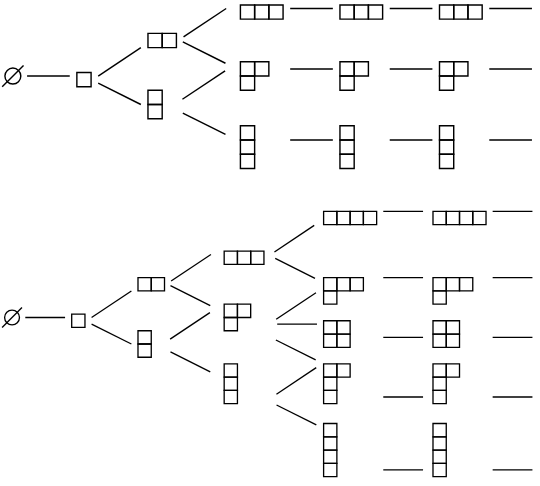
\includegraphics[width=9cm]{xfig-ppm/rollet.png}

\caption{\label{fig:R2}  The Rollet graphs/diagrams  $\Roll_{-1}$, 
$\Roll_1$ and   $\Roll_2$.  
(See \ref{ss:gdetl0} for $\Roll_0$.)
\\
In $\Roll_2$, for example, the head of the graph is the first five columns; 
with the \hip\ being the 5th column; and columns five and above being the \arm s. %\bajm{[small error - the column has 5 boxes but should have 4]}\ppm{[fixed.]}
}
\end{figure} 

%Similarly for $J_{1,n}$ we have $\Roll_1$:

%\includegraphics[width=9cm]{xfig-ppm/rolletJ0.eps}

\medskip \medskip 

The Rollet graph encodes standard module restriction rules - specifically filtration factors. 
Thus in particular we have the following. 

\mdef   \label{pr:walks0}
The dimension of the standard module of $J_{l,n}$ with label 
$v=(p,\lambda)$ is given by the number of walks of length $n$ from $\emptyset$ to $v$ 
 %$\lambda$ 
on the graph $\Roll_l$. 



%\newcommand{\boxx}{\!\!\!\!\qed\;}  %% ugly hack!

\mdef 
\ignore{{ 
For completeness (and also to facilitate the making of a useful point) let us include the case 
$\Roll_{-1}$, 
for $J_{-1,n}$:

\medskip 

\beq %$
\emptyset - \boxx -\boxx -\boxx - ...
%$...   
\eq 
\medskip

\noindent 
}}
In the $l=-1$ case, $p$ determines $(p,\lambda)$, so we can use just $p$ for the label.
Walks of length $n$ from 0 (i.e. $(0,\emptyset)$) to $p$  (i.e. $(p,\boxx)$)
on this $\Roll_{-1}$ graph can be used to give a basis for the corresponding 
Temperley--Lieb standard module (indeed there are multiple distinct useful such bases). 
From this, or directly, we can give a corresponding matrix representation from which, in turn, we can start to see the role of alcove geometry in this setting (alcove geometry, particularly type affine-$A_1$ --- affine reflection groups on the line, arises naturally in Lie representation theory and hence can be considered to arise here via Schur--Weyl duality, but we can also understand it directly). 

%\bajm{[?? not finished]}\ppm{[enough for now?]} 
The construction is as follows  \cite{Martin91}. % for details). 
First we consider our graph as embedded in $\R$ so that the vertices are a subset of the integral points:
then walks on the embedded graph from 0 to $\l$ are put in correspondence with bases (in various ways - see \S\ref{ss:gdTL}) for the $\l$ standard module. 
In a suitable bases there is a decoupling of walks exceeding a geometrical bound when $\xx$ is the root of a Chebyshev polynomial - a submodule, and hence giving a map in from another standard module, say $\l'$. The map in can be organised as the label $\l'$ being the image of $\l$ under the action of a suitable realisation (depending on $\xx$) of the affine reflection group. See \S\ref{ss:repthy} for visualisations. 
%...

%As we will see \ppm{when [!]} the details above are added, the Chebyshev polynomials play, in a sense, two roles there. At the other extreme (large $l$) one can compare with \cite{DeVisscherMartin2016} ...  (in particular there we have the King polynomials - in just one of the two roles played by Chebyshev polynomials above ...) ...

%\mdef  \ppm{And finally let us include $l=0$. [and at least run a bit of combinatorics? - see (\ref{pa:l0OEIS})]} 


\ignore{{
\mdef  \ppm{[DELETE this para, or at least delete ref to C1, for now.]}
Later, in \S\ref{ss:walkbases0}, 
we will describe bases for $\Deltaa$-modules in terms of walks on Rollet graphs,
and hence more `geometrical' than diagram bases. And hence potentially better suited to extending the corresponding known bases in case $l=-1$.  
}}

%
\subsection{On walk bases for $\Delta$-modules for $l\geq 0$}
\label{ss:walkbases0}

We can go further than the combinatorial correspondence in (\ref{pr:walks0}). 
\ppm{[-can we actually?!  there is a lot of colour here.  might minimize this section for the first submission???]}

\mdef   Example. 
%\bajm{\sout{I have so far counted 13 walks of length 5 from $\emptyset$ to $(2,1)$, but in my calculation it has dim 14... I must be missing a walk...} got it!} 
Formally, 
%OK let's make a start on writing 
the walk-basis for 
$\Delta^{l=1}_{5,((21),0)}$    %in \bajm{( understood :) )}
is:
\begin{equation}  \label{eq:walkbasis521}
0-1-0-1-(2)-(21),
\;\;\; \;\;\; \hspace{.421cm}
0-1-0-1-(11)-(21),  \hspace{2.29762cm} 
\end{equation}
\[ 
0-1-(2)-1-(2)-(21),
\;\;\; \hspace{.31cm} 
0-1-(2)-1-(11)-(21),   \hspace{.53cm} 
\;
0-1-(11)-1-(2)-(21),
\] 
\[ 
0-1-(11)-1-(11)-(21),  \;\;\;
0-1-(2)-(21)-(2)-(21), \;\;\;
0-1-(2)-(21)-(11)-(21),
\]
\[ 
0-1-(2)-(21)-(21)'-(21), \hspace{1.9753185cm} 
0-1-(11)-(21)-(2)-(21), \hspace{.2cm} 
\]
\[ 
0-1-(11)-(21)-(11)-(21),  \;\;\; \hspace{1.95cm} 
0-1-(11)-(21)-(21)'-(21),
\]
\[ 
0-1-(2)-(3)-(2)-(21), \;\;\; \hspace{.96cm} 
0-1-(11)-(111)-(11)-(21)
\]

\mdef   \label{exa:l0p6la2}
Example. 
Explicit partial bases for  
$\Deltaa^{l=0,n=6}_{(4,(2))}$ is:  %and ... (not consistent with proper labelling \ppm{yet!}):  
\medskip 

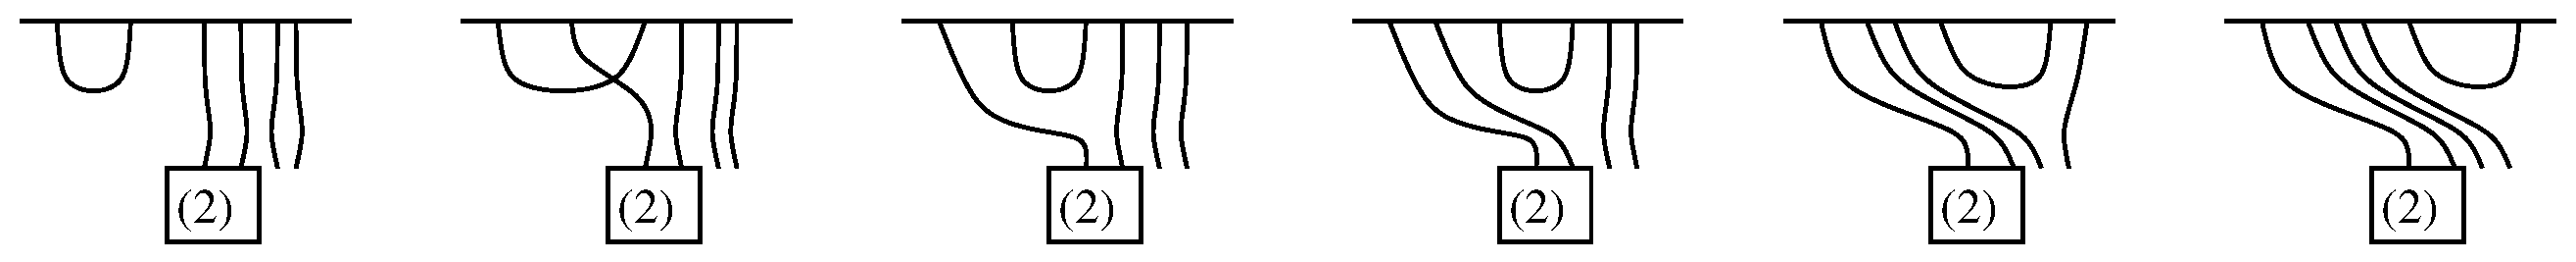
\includegraphics[width=10.9cm]{xfig-ppm/Delta62bas.eps}

\ppm{[So far the following is nonsense, but at least there are pics of diagrams. I'll fix it!...]}
The elements expressed as walks (writing $\lambda'''$ to mean $(\lambda,3)$ and so on):
\begin{align*}
    &0-1-0-1-(2)-(2)'-(2)''& &\sim e_{1,2}, \\
&0-1-(2)-1-(2)-(2)'-(2)'' &&\sim e_{2,3}, \\
&0-1-(11)-1-(2)-(2)'-(2)'' &&\sim e_{1,3}, \\
&0-1-(2)-(2)'-(2)-(2)'-(2)''&&\sim e_{3,4}, \\
&0-1-(2)-(2)'-(2)''-(2)'-(2)''&&\sim e_{4,5}, \\
& 0-1-(2)-(2)'-(2)''-(2)'''-(2)'' &&\sim e_{5,6},\end{align*}
(finish me!... \bajm{right? I am also suggesting the above correspondence with diagrams} \ppm{[-interesting. does that represent the application of an algorithm, or so far just a one-off?
For $l=-1$ of course the Rollet graph is just a simple chain $0-1-1'-1''-...$ which we could also label as $0-1-2-3-...$. There is a natural partial order on walks of length $n$ from 0 to (say) $s$, with $0-1-0-1-...-0-1-2-3-...-s$ the lowest and $0-1-2-...-max-...-(s+1)-s$ the highest. One can assign the diagram cup-cup-...-cup-line-line-...line to the lowest; and then construct the others iteratively so that if walk $w'$ is obtained from $w$ by $j-(j-1)-j \;\leadsto\; j-(j+1)-j$ (for some $j$) in position $i$ then the diagram $d'$ is given by $U_i d$. Does that make sense? (There is a more complicated version for Brauer. If we are lucky the general $l$ case (or at least some intermediate $l$ case) might be easy to interpolate.  - In which case this might even make the germ of a neat little paper.)]}\bajm{I think this represents the application of an algorithm which I don't quite understand yet :)... but seems quite accesible}). 


Aside. Here is another set of walks (for a different module! \bajm{for $\Delta^{l\geq 0}_{6,((2),0)}$ ?}):
\begin{align*} 
&0-1-0-1-0-1-(2), &&
0-1-0-1-(2)-1-(2),\\
&0-1-0-1-(11)-1-(2),
&&0-1-(2)-1-0-1-(2),
\\ &0-1-(2)-1-(2)-1-(2),
&&0-1-(2)-1-(11)-1-(2),
\\ &0-1-(11)-1-0-1-(2),
&&0-1-(11)-1-(2)-1-(2),
\\&0-1-(11)-1-(11)-1-(2).\end{align*}
(Is this correct?! \bajm{There should be more walks no? None of these walks go past $(2)$ in the rollet graph} \ppm{[-yes agreed. (I'm working in spurts as pain levels allow, so there'll be some mud in my tex-ing waters. hopefully more good than bad overall.  :-) )]})



\medskip  \noindent  Another example is
$\Delta^{l=1}_{4,(2)}$:  \medskip 

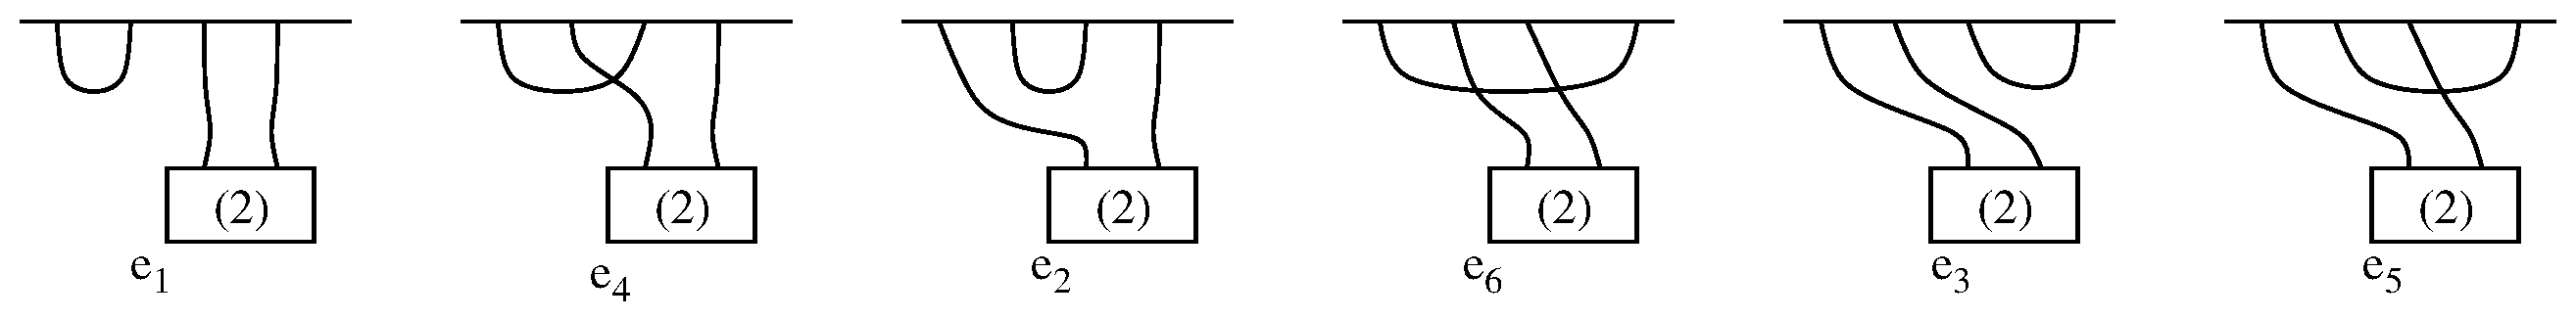
\includegraphics[width=10cm]{xfig-ppm/Delta42bas.eps}

The elements expressed as walks:  
\begin{align*}
    &0-1-0-1-(2), &&\sim e_{1,2}, &&0-1-(2)-1-(2),  &&\sim e_{2,3}, \\
&0-1-(2)-(3)-(2), &&\sim e_{3,4}, &&0-1-(2)-(21)-(2), &&\sim e_{2,4},\\
&0-1-(11)-1-(2), &&\sim e_{1,3}, &&0-1-(11)-(21)-(2), &&\sim e_{1,4}.
\end{align*}

\bajm{Next look at $\Delta^{l=1}_{6,((3),1)}$, $\Delta^{l=2}_{6,((4),0)}$... See if this sheds light on walk $\to$ diagram map:}
For $\Delta^{l=1}_{6,((3),1)}$, in addition to the walks included in the $l=0$ cases (now replacing $(2)^{'}$ with $(3)$, $(2)''$ with $(3)'$  etc) we also include:
\begin{align*}
    &0-1-(11)-(21)-(2)-(3)-(3)' &&\sim e_{1,4}, \\
&0-1-(2)-(21)-(2)-(3)-(3)'&&\sim e_{2,4},
\end{align*}

For $\Delta^{l=2}_{6,((2),2)}$ we include the previous walks (replacing $(3)'$ with $(4)$) and we include:
\begin{align*}
    &0-1-(11)-(21)-(31)-(3)-(4) &&\sim e_{1,5}, \\
&0-1-(2)-(21)-(31)-(3)-(4)&&\sim e_{2,5},\\
&0-1-(2)-(3)-(31)-(3)-(4)&&\sim e_{3,5},
\end{align*}
\bajm{I seem to be on the verge of being able to formulate a correspondence between walks and diagrams, at least in the case of 1D Specht-modules, by considering the positions of ``turnbacks" and ``deviations" from an ``ideal walk" (ideal walks i am tentatively defining as those which consist only of subdiagrams of the final diagram (need to modify to deal with going to right of final diagram...) ).   }


%
\section{Young Graph by Alcove Geometry}
This section is a small note, devoted to the idea of realising the Young Graph by alcove geometry. Firstly, consider the type $B_{\infty}$ Weyl group, $G$:
\[ G=\langle s_0, s_1,\dots \ | \ s_k^2=(s_0 s_1)^4=(s_{l}s_{l+1})^3=(s_i s_j)^2=e \ \text{for }l>0, |i-j|>1 \rangle,\]
acting on $\R^\infty$ (the space of finite real sequences) as follows:
\begin{align*}
    s_0(x_1,x_2,\dots,x_n)&=(-x_1,x_2,\dots,x_n),\\
    s_i(x_1,\dots,x_i,x_{i+1},\dots,x_n)&=(x_1,\dots,x_{i+1},x_i,\dots,x_n),
\end{align*}
where we use $(x_1,x_2,\dots,x_n)$ as short hand for the same infinite sequence, padded by 0s on the right. By allowing the $x_k$ to possibly be 0, we can ensure the last definition is always sensible. We can consider the $s_0$ as acting by reflection in the hyperplane defined by $x_1=0$, and the $s_i$ as acting by reflection in the hyperplane defined by $x_i=x_{i+1}$.

Given an element $(x)\in \R^\infty$ we can apply $s_0$ (conjugated by permutations to act in each component) so that all non-zero elements are positive, and then apply a permutation to order all entries in descending order. Thus a fundamental domain, $\mathcal{D}$, for $G\circlearrowright \R^\infty$, is the set of finite, descending, positive sequences:
\[\mathcal{D}= \left\{(x_1,x_2,\dots, x_n,0,\dots) \in \R^\infty \ \Bigg| \ \begin{matrix}\text{ for some } n\in \N \text{ such that }\\ x_1\geq x_2\geq \dots \geq x_n>0\end{matrix} \right\}.\]
Now, let us augment our group to be $\hat{G}$ where we add another generator $r_0$ to $G$ which satisfies the exact same relations as $r_0$ and has no ``braiding" relation with $s_0$. We give a Dynkin diagram for the group $\hat{G}$ below:
\[ \begin{tikzcd}[column sep=tiny,row sep = tiny]
    s_0\ar[dr,equal]\\
    &s_1\ar[r,dash]&s_2\ar[r,dash]&s_3\ar[r,dash]&\dots\\
    r_0\ar[ur,equal]\ar[uu,dash,"\infty"]
\end{tikzcd}\]
Now let $r_0$ act on $\R^\infty$ by the (affine) reflection in the hyperplane defined by $x_1=1$, that is,
\[r_0(x_1,x_2,\dots,x_n)=(2-x_1,x_2,\dots,x_n).\]
We then observe that $r_0 s_0$ acts by $x_1\mapsto x_1+2$ (fixing all other components). For a partition, $\l\vdash n$, we may view $\l=(\l_1,\l_2,\dots, \l_r)\in \mathcal{D}$ with $\l_i\geq \l_{i+1}$ for all $i$. Now define
\[\mathcal{D}_{\l}:=\{x\in \R^\infty \ | \ x-\l \in [0,1)^\infty  \}.\]
Clearly $\mathcal{D}=\sqcup_{\l} \mathcal{D}_{\l}$ and furthermore, we claim that each $\mathcal{D}_{\l}$ is a fundamental domain for $\hat{G}\circlearrowright \R^\infty$ (or an alcove) which shares a face with $\mathcal{D}_{\l'}$, if and only if, $\l'$ is a partition obtained from $\l$ by ``adding or removing a box". Suppose that $\l$ and $\l'=(\l_1,\dots,\l_i+1,\dots ,\l_r)$ are both partitions. Then $\mathcal{D}_{\l}$ and $\mathcal{D}_{\l'}$ (or rather, their closures) share the face
\[\overline{\mathcal{D}_{\l}}\cap\overline{\mathcal{D}_{\l'}}=\left\{\begin{matrix}(\l_1+\xi_1,\dots,\l_i+1,\dots,\l_r+\xi_r,\xi_{r+1},\dots,\xi_k)\in \mathcal{D}  \\ :\text{for some } k \in \N, \text{ where } \xi_l\in [0,1]\end{matrix} \right\}.\]
Therefore, by identifying each alcove $\mathcal{D}_{\l}$ with the underlying partition $\l$, we obtain the Young-graph as the dual graph of this alcove geometry.


   %% modularised into a file for ease of movement
%% ...and moved to the end of doc for now
  
